\documentclass{article}
\usepackage{graphicx}

\date{\today}
\author{Tarik Atlaoui \\ Nicolas Peugnet \\ Kimmeng Ly \\ Max Eliet}

\begin{document}


\begin{titlepage}
	\enlargethispage{2cm}
	\newcommand{\HRule}{\rule{\linewidth}{0.5mm}}
	\center
	\textsc{\LARGE
	Carnet de bord du PSAR 
	} \\[1cm]
	\HRule \\[0.4cm]
	{ \huge \bfseries API générique pour le développement d'applications réparties \\[0.15cm] }
	\HRule \\[4cm]
	\large{Tarik Atlaoui \\[3mm] Nicolas Peugnet \\[3mm] Kimmeng Ly \\[3mm] Max Eliet} \\[3cm]
	09 Mars 2020 \\[3cm]
	\hfill 
\includegraphics[width=5cm]{logoSU.jpg}
\end{titlepage}

	\newpage
	\pagenumbering{arabic}
		\section{Introduction}
			\large{
			\indent Aujourd'hui la vaste majorité des applications en fonctionnement sont des applications qui sont déployées dans un contexte distribué, c'est a dire qu'elles
			ne sont pas juste hébergées sur un serveur et n'ont besoin que de ce dernier afin de fonctionner. Au contraire, elles sont déployées sur une multitude de serveurs, de base de données et autres 
			qui eux même sont dupliqués afin de s'assurer que même en cas de panne l'application ne cessera pas de fonctionner.
			Cependant, ce type d'applications est extrêmement dur à développer car on ne peut pas les tester dans des conditions réelles et souvent le code écrit pour un simulateur 
			n'est pas le même que celui ecrit pour le déploiement.
			Elles sont aussi difficiles à maintenire car entre autres les mises à jour doivent être propagées à toutes les machines. Enfin, leur débogage est complexe car même lorsque l'application
			fonctionne normalement, elle n'a pas un comportement déterministe dû à son fonctionnement réparti.
			\indent C'est dans ce contexte que notre projet prend place et a pour but d'implémenter un intergiciel permettant l'execution d'applications réparties, aussi bien sur une infrastructure réelle que sur un simulateur, sans avoir à en modifier le code, afin de simplifier le développement de futures applications réparties.
\\[2mm]
			 \indent Dans notre cas, nous avons choisi d'implémenter cet intergiciel pour MPI (Message Passing Interface) en tant qu'API d'infrastructure réelle, et PeerSim en tant que simulateur à événements discrets.}
		
		\section{Les mots clés retenus}
		-PeerSim
		\newline
		-MPI
		\newline
		-Message Passing Interface
		\newline
		-Distributed systems
		\newline
		-p2p simulator
		\newline
		-Simulation of Distributed systems
		\newline
		-distributed algorithms
		\newline
		-Naimi and Trehel algorithm
		\newline
		-Ring algorithm
		\newline 
		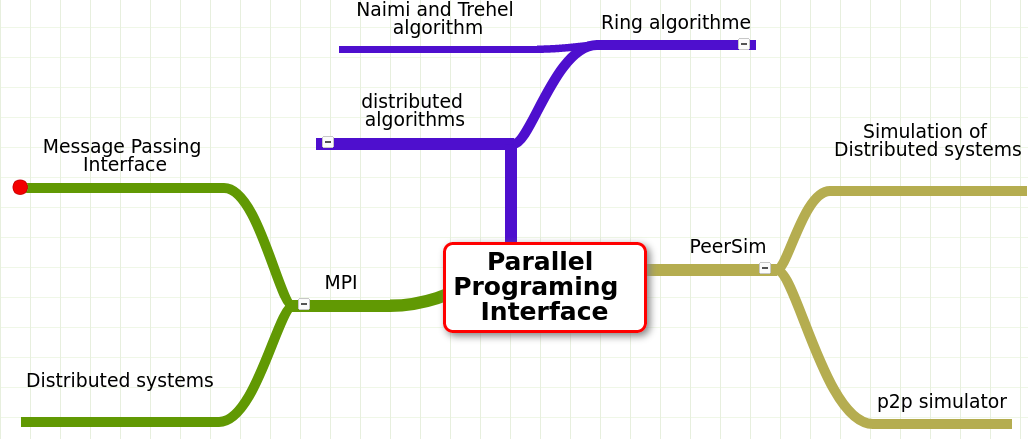
\includegraphics[width=10cm]{mindmap.png}
		\newpage		
		\section{Descriptif de la recherche documentaire}
		\indent Nous avons commencé par comprendre ce qu'est un systeme distribué et comment fonctionnent les systemes MPI et PeerSim à travers quelques exemples d'algorithmes que nous avons implémenté dans chacune des API. 
		\newline
		\indent	
Nous avons aussi utilisé google scholar pour comprendre comment la communauté utilise les deux API, ainsi que pour avoir la version exacte et prouver des algorithmes que nous avons utilisé car pour les algorithmes il est facile de passer à côté et beaucoup de gens implémentent des versions fonctionnelles mais qui n'appliquent pas vraiment l'algorithme.
		\newline
		\indent
 C'est pour ces raisons que, pour les deux API, nous avons utilisé les documentations des developpeurs qui ont créé les deux API pour mieux comprendre les subtilités de celles-ci.
		\newline
		\indent Nous avons beaucoup utilisé google scholar car il a une quantité impressionante de ressources et qu'elles sont pour la plupart des sources fiables et cela nous a permis d'acceder aux thèses qui nous intéressaient, aussi nous avons utilisé la doc du langage Java , puisque ça a été le langage d'implantation de notre interface.

		\newpage
		\section{Bibliographie produite dans le cadre du projet}

		[1]    « PeerSim P2P Simulator ». [En ligne]. Disponible sur http://peersim.sourceforge.net/#docs.
		\\[2mm]		
		[2]    « Open MPI Documentation ». [En ligne]. Disponible sur: https://www.open-mpi.org/doc/.       
		\\[2mm]			
		[3]          J. Lejeune, « TME ARA PeerSim : Prise en main ».
		\\[2mm]		
		[4]    S. Morin, I. Koren, et C. M. Krishna, « JMPI: Implementing the message passing standard in Java », in Proceedings 16th International Parallel and Distributed Processing Symposium. IPDPS 2002, 2002, p. 6–pp.          
		\\[2mm]	
		[5]    B. Carpenter, G. Fox, S. H. Ko, et S. Lim, « Object serialization for marshaling data in a Java interface to MPI », Concurrency: Practice and Experience, vol. 12, no 7, p. 539–553, 2000.
		\\[2mm]		
		[6]          I. Kazmi et S. F. Y. Bukhari, « PeerSim: An Efficient Scalable Testbed for Heterogeneous Cluster-based P2P Network Protocols », in 2011 UkSim 13th International Conference on Computer Modelling and Simulation, 2011, p. 420–425. 
		\\[2mm]		
		[7]          A. Jodoin et M. Desmarais, « L’environnement de développement dynamique (EDD) pour le prototypage rapide d’interfaces graphiques », in Proceedings of the 21st International Conference on Association Francophone d’Interaction Homme-Machine, Grenoble, France, 2009, p. 111–117. 
		\\[2mm]
		[8]       M. Baker, B. Carpenter, G. Fox, S. Hoon Ko, et S. Lim, « mpiJava: An object-oriented java interface to MPI », in Parallel and Distributed Processing, Berlin, Heidelberg, 1999, p. 748–762.
		
		\newpage
		\section{Evaluation des sources}

		\\[2mm]
		[2] Documentation MPI : En tant qu’étudiants en Master Informatique nous avons eu l’occasion d’utiliser une multitude d’outils et de langages de programmation mais nous avions pas encore eu l’occasion de manipuler l’API Mpi. Et la documentation est un outil important pour pouvoir comprendre son fonctionnement et son utilisation. C’est la documentation officielle ecrite par les hauters de l'api, il n’y a donc aucun doute à avoir sur son contenu.
		\\[2mm]
		[4] S. Morin, I. Koren, et C. M. Krishna, « JMPI: Implementing the message passing standard in Java », Dans le cadre de notre projet, nous devons utiliser le langage Java pour faire le lien entre l’API Mpi et celui de PeerSim. Ce guide  correspond exactement à ce dont nous avons besoin, en effet il permet d’en apprendre plus sur le déploiement des services offerts par l’API Mpi et ainsi de les utiliser dans le langage Java.
		\\[2mm]
		 [3] J. Lejeune, « TME ARA PeerSim : Prise en main »,  Ce TME, qui nous a été fourni par notre encadrant, nous a permis à comprendre comment fonctionne Peersim. Nous avons, grâce à ce tuto, pu se “familiariser avec l’API de l’outil PeerSim en implémentant un protocole simple” qui consistait à envoyer un message contenant des données simples d’un noeud vers un autre.

\end{document}
